\section{Билет 8. Создание СССР и национально"=государственное строительство в 1922--1936гг}

\subsection{Первые автономии.(наверное лучше так оставить)}

Ещё в декабре 1917 года была признана независимость Финляндии. Независимость Польши была подтверждена в Рижском мире 1921 года. Была признана независимость Литвы, Латвии и Эстонии.

\subsection{Возникновение новых гос образований в годы Гражданской войны и предыстория создания СССР.}

В июле 1918 года была принята первая советская конституция, в которой Россия объявлялась республикой советов, а второй статьёй Российская советская республика определялась как федерация советских национальных республик. Федеративное устройство предусматривало автономию различных республик. Они возникают в годы гражданской войны.

Первой в 1918 году такой стала трудовая коммуна немцев Поволжья.

В 1919 году появилась Башкирская республика на Южном Урале. В среднем Поволжье татарская республика, Чувашская и Марийские республики. В низовьях волги "--- Калмыцкая.

В 1921 году на северо"=западе страны была создана Карельская трудовая коммуна. После того, как войска заняли Крымский полуостров, там создаётся Крымская советская социалистическая республика. 

Дальше продолжили появляться автономии на ближнем востоке, сибири.

Кроме того, появляются Украинская ССР, Белорусская ССР. В закавказье "--- Армянская, Грузинская и Азербайджанская ССР. Все эти республики связаны с РСФСР военно-политическими договорами.

\subsection{План федерализации и автономизации.}

К моменту окончания гражданской войны начинаются обсуждения по поводу пост"=военного государства. 

Создаются два варианта развития страны:

\begin{enumerate}
    \item Ленин: «План федерализации страны». Будущее советское государство будет выглядеть как федерация республик с максимально широко определенными правами и правом на отделение от РСФСР
    \item Сталин: «План автономизации». Все республики войдут в состав РСФСР на правах национально-культурных автономий без права на отделение.
\end{enumerate}

В  течение 21--22 году велись споры по принятию плана. По форме был принят Ленинский план, однако по содержанию это был Сталинский.

\subsection{Первый союзный договор и Декларация об образовании СССР.}

30 декабря 1922 года на конференции делегации от съездов Советов четырёх республик принимают декларацию об образовании СССР. В состав входят РСФСР(Русская советская федеративная социалистическая республика), УССР(Украинская советская социалистическая республика), БССР(Беларусская советская социалистическая республика), ЗСФСР (Закавказская советская федеративная социалистическая республик).

\subsection{Принятие конституции 1924 года.}

\subsubsection{\textbf{Про конституцию (принятие, разделы).}}
В 1924 году на следующем съезде принята конституция СССР. Это конституция провозгласила союз свободный и равноправный федерации (?). Первый раздел "--- декларация об образовании союза советских социалистических республик, а вторая часть "--- договор об образовании СССР. Статья 4 гласила, что за каждой республикой оставляется право свободного выхода из союза. Другие статьи описывали структуру органов власти. Верховным органом власти провозглашался съезд советов (как и раньше, с 1917 года), а в период между схездами "--- центральный исполнительный комитет (ЦИК). В отличие от более ранней модели он делился на две палаты: Совет союза и совет национальностей. Они формировались по"=разному. Сам съезд формировался выборами на местах, а в ЦИК(центральный исполнительный комитет) попадали представители союзных республик из совета союза. Количество было пропорционально населению республики.

\begin{figure}[H]
    \centering
    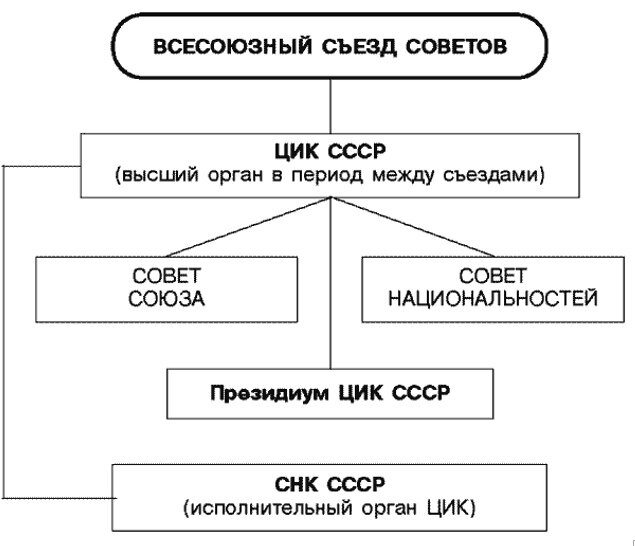
\includegraphics[width=0.7\textwidth]{картинки/Структура_власти_1924.jpeg}
    \caption{Структура советской власти, согласно конституции 1924 года.}
\end{figure}

\subsubsection{\textbf{Про совет национальностей.}}

В совет национальностей из каждой союзной республики попадали по 5 депутатов, но кроме того, туда попадали и представители автономий. Таким образом хотели объединить многонациональный характер страны и централизованное принятие решений.

\subsubsection{\textbf{Про Всесоюзный съезд, ЦИК и тд.}}

Всесоюзный съезд советов был высшим органом власти, а ЦИК от себя избирал президиум и совнарком "--- высший исполнительный орган. Высшим судебным органом по конституции становился верховный суд. В каждой из союзных республик создавалась своя структура, полностью копирующая структуру власти СССР.

В 19 статье конституции говорилось, что все декреты принятые ЦИК исполнялись на всей территории СССР.

\subsubsection{\textbf{Про ВКП(б).}}

Всесоюзная коммунистическая партия большевиков (ВКПБ). Они вырабатывают все решения, которые потом реализуются исполнительными органами. В конституции о роли партии ничего не говорилось, но на практике ещё со времен гражданской войны произошло сращение государственного аппарат и партии. Большинство дореволюционных партий объявляются вне закона, уничтожаются меньшевистские и эсеровские организации.

\subsubsection{\textbf{Про ЦК РКП(б).}}

Подлинно руководящим центром партии являлся её центральный коммитет (ЦК РКП(Б)), но из этой структуры выделялось Политбюро, куда входили самые влиятельные лидеры. Именно это Политбюро при центральном коммитете вырабатывало все важнейшие решения. Туда входили Ленин, Сталин, Зиновьев, Каменев и Троцкий. Бухарин, Калинин и Молотов "--- кандидаты, которые могли присутствовать на заседаниях, обсуждать решения, но не имели права голоса.

Таким образом государство, именовавшееся федеративным, являлось по сути унитарным.

\subsubsection{\textbf{ОГПУ.}}

По конституции провозглашалось создание при совнаркоме объединенного государственного политического управления (ОГПУ). Оно создавалось «в целях объединения революционных усилий союзных республик для борьбы с контрреволюционным движением, шпионажем и бандитизмом». То есть ОГПУ заменило существовавший ранее ВЧК. Хотя люди остались те же (Дзержинский "--- лидер ВЧК и теперь ОГПУ).

\subsection{Политика коренизации советской власти и борьба по вопросу о национальном строиельстве.}

После принятия конституции национальное государственное строительство выражалось созданием автономий внутри республик, а также в дальнейшем некоторые автономные республики добивались более высокого статуса и превращались в союзные республики. Так в 1924 г. союзными стали Узбекская и Туркменская республики. Также Таджикская ССР. Киргизская и Казахские ССР в 1936 году также стали союзными республики, когда принималась новая конституция СССР.

\subsubsection{\textbf{Коренизация.}}

Формирование новых автономных/союзных республик сопровождалось политикой коренизации. Она выражалась в подготовке и выдвижении в правительство представителей коренных народов. Также она выражалась во внедрении языков национальных меньшинств. В документооборот, образование. Коренизация выражалась в поощрении издания газет, журналов на местном языке. Появлялись культурные организации в каждом регионе.

\subsection{Новая конституция("Сталинская").}

\subsubsection{\textbf{Сталинская конституция}}
В начале 1930"=х годов в среде советского руководства появляется мысль о переработке конституции. Её старая версия, появившаяся еще в период гражданской войны не соответствовала потребностям строительству социализма и в период 1930"=х годов произошла смена политического курса. Нужно было сосредоточиться на защите собственных интересов. С инициативой закрепить изменения в новом варианте конституции выступил Сталин. В течение двух лет (1934 и 1936 г.) велось обсуждение конституции. В результате, 5 декабря 1936 года принимается новая конституция СССР. 

\subsubsection{\textbf{11 республик СССР.}}
Она зафиксировала, что в составе союза 11 республик (РСФСР, БССР, УССР, Казахстан, Туркменистан, Киргизия, Таджикистан, Грузинская, Азербайджанская, Армянская, Узбекская). Внутри этих республик продолжали существовать автономные республики. В РСФСР – карельская, чувашская, башкирская, автономная республика немцев Поволжья (переименованная трудовая коммуна немцев), Калмыцкая, Дагестанская, Чеченская, Ингушская, Кабардино-Балкарская, Коми, Якутская, Бурятская, Хакасская, Крымская, и др.

В составе УССР И БССР автономий тогда не было.

\subsubsection{\textbf{Изменения в структуре органов власти.}}

Новая конституция несколько изменила структуру органов власти. Высший законодательный орган власти теперь называется Верховный Совет СССР (Вместо съезда советов). Он избирался населением страны каждые 5 лет. Каждый раз был блок коммунистов и беспартийных. Верховный совет состоял из двух равноправных палат (Совет союза и совет национальностей, формировались по прежним принципам). Он избирал президиум верховного совета, избирал правительство (называвшиеся Советом народных комиссаров СНК), и генерального прокурора. Оформлял в виде указов принятые решения.
В новой конституции в 126 статье закреплена роль партии. 

\begin{figure}[H]
    \centering
    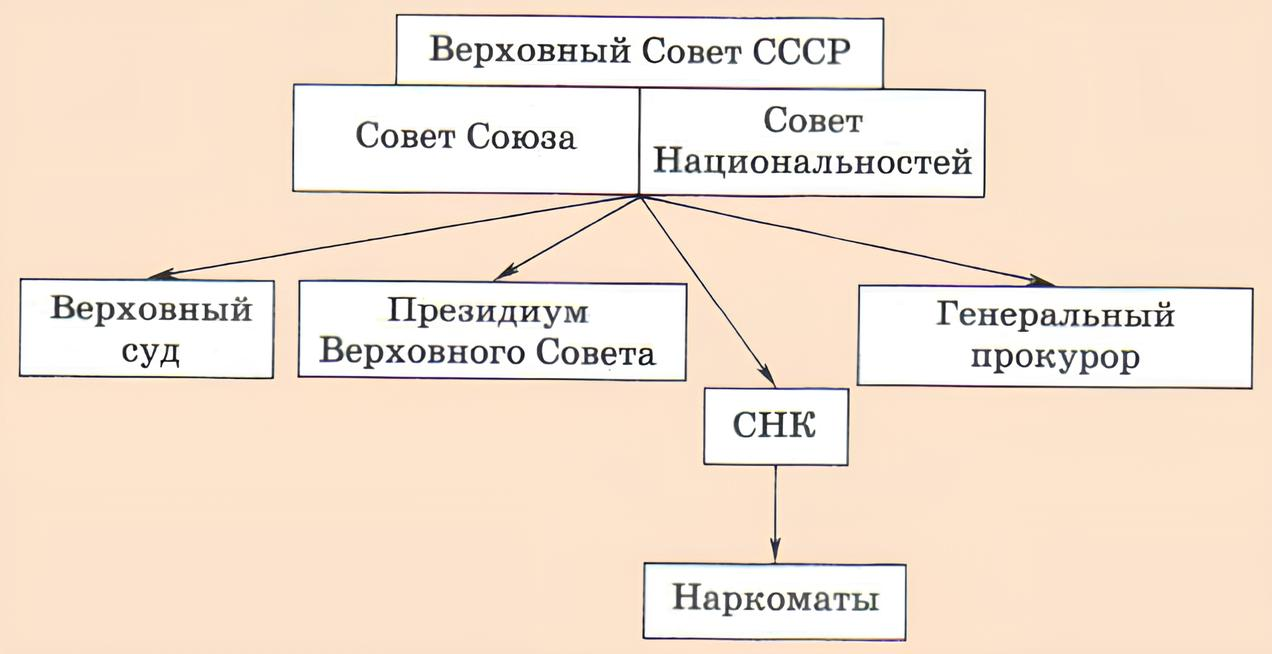
\includegraphics[width=0.8\textwidth]{картинки/Структура_советской_власти_1936.jpg}
    \caption{Структура советской власти, согласно конституции 1936 г.}
\end{figure}

\subsubsection{\textbf{Структура партии.}}

Структура партии (снизу вверх):

\begin{itemize}
    \item Первичные партийные организации (занимались приёмом в партию, рассматривали вопросы на повестке дня, которые отправлялись с верху, к примеру, вопрос о принятии новой конституции)(уездные, волостные, городские коммитеты партии).
    \item Территориальные коммитеты партии.
    \item Съезд РКП(б) (высший орган руководства партией). 
    \item Центральный комитет (ЦК РКП(б)) (постоянный руководящий орган партии).
    \item Политбюро.
\end{itemize}

Параллельно политбюро существовали Оргбюро и Секретариат ЦК РКПБ(б).

\subsubsection{\textbf{Немного про президиум.}}

Между сессиями верховного совета президиум становится высшим распорядителем. На практике в совет президиума избирались те же люди, которые входили в секретариат ЦК ВКПБ. Он регулировал жизнь государства и потому функции президиума постоянно расширялись. Среди возможностей президиума "--- объявление военного положения, принятие в гражданство, контроль подотчётных органов, издание подзаконных актов.